\documentclass[11pt,a4paper]{article}   

\usepackage[margin=1.0in]{geometry}

\usepackage{graphicx}
\graphicspath{ {./figures/} }
\usepackage{floatrow}
\usepackage{subfig}

\usepackage{amsmath}
\usepackage{comment}

\newcommand\RE{\operatorname{Re}} 
\newcommand\IM{\operatorname{Im}} 
\newcommand\Tr{\operatorname{Tr}} 

\newcommand\MSbar{$\overline{\text{MS}}$ } % MS-bar 
\newcommand\he[1]{#1^\dagger}% Hermitian conjugate
\newcommand\gr[1]{\mathrm{#1}}% font for group names such as SU(2)


\usepackage{color}
\definecolor{myorange}{rgb}{1,0.5,0}
\newcommand\lauri[1]{{\color{myorange}#1}}

\title{Basic documentation for lattice simulations}
\author{Lauri Niemi}
\date{\today}

\begin{document}
\maketitle


\section{Multicanonical algorithm}

In a first-order phase transition, mixed-phase configurations are exponentially suppressed by a factor proportional to the volume, $p \sim e^{-V}$. Thus, for large lattices it becomes necessary to enhance tunneling probability in order to study phase transitions. For this we use the multicanonical method \cite{Berg:1991cf}: our action is modified by a weight function $W(R)$, where $R$ is a suitable order parameter that distinguishes all relevant phases. We choose sign convention $S' = S_\text{canonical} + W(R)$, so that weight \textit{increases} when a certain configuration is to be suppressed and the ideal weight function is just the canonical probability distribution for $R$. Once we obtain a multicanonical distribution from a simulation, the canonical distribution is obtained simply by reweighting. \textbf{In the measurement file, we measure $-W(R)$ instead of $W(R)$ to ensure compability with Kari.}

In practice the weight function is implemented by specifying a range $R_\text{min} \leq R \leq R_\text{max}$ that we want to enhance with multicanonical, and dividing this range into bins of equal length so that the system is in bin $i$ when $R_{i} \leq R < R_{i+1}$, and $R_0 = R_\text{min}$. Inside bin $i$, we approximate $W$ by a linear interpolation. Denoting $W(R_i) = w_i$, for $R_{i} \leq R < R_{i+1}$ we have 
\begin{align}
W(R) = w_i + (R - R_i) \frac{w_{i+1} - w_i}{R_{i+1} - R_i},
\end{align}
and in the last bin we simply use constant weight. Outside the binning range the weight is chosen to be constant and equal to $w_i$ in the nearest bin. \lauri{For nucleation we would need infinite weighting outside the range. This is also implemented and can be specified in config file.}

Since the weight function generally depends on a \textit{global} parameter $R$ (ex. volume average of $\phi^\dagger\phi$), parallelization of multicanonical algorithms is not straightforward. We use the following method, adapted from Kari: 

\begin{itemize}
	
	\item Perform an even-odd sweep on the lattice, updating half of the sites locally using \textit{canonical} updates such as overrelaxation. This moves the system towards a local minimum of the canonical ensemble. For example if the order parameter is $\phi^\dagger\phi$, we update the Higgs field at half of the sites but do not touch the other fields yet.
	
	\item After the sweep, recalculate the order parameter and perform an accept/reject step based on the change in the weight function. The sweep of updates is accepted with probability $\min(1, \exp[W(R) - W(R') ])$, where $R$ and $R'$ are the old and new values the order parameter. If rejected, ALL local updates contributing to the weight change are undone (ex. if $R$ is the Higgs hopping term, we sweep and update gauge links and the Higgs, and then apply the multicanonical step. If rejected, undo changes in both Higgs and the links). This step produces a bias towards mixed-phase configurations where the weight function is smaller. 
	
\end{itemize}

For the "easy" order parameter $\phi^\dagger\phi$, the acceptance rate of the multicanonical update is generally good, $>90\%$. This is in agreement with Kari's acceptance rates in the SM and MSSM. \textbf{To do:} optimize the algorithm for more complicated order parameters. It should be safe to do perform the multicanonical step in parts, so that if we choose hopping term as the order parameter, we can first update half of the links, do global acc/rej, then update half of the Higgs and do acc/rej again etc.

\subsection{Calculation of the weight function}

Since the canonical probability distribution (and the weight) is not known \textit{a priori}, we need an algorithm for approximating the weight function. For our purposes there are (at least) two good options for automatizing this process: 
\begin{itemize}
	
	\item Recursive computation of Berg. The detailed recipe for performing (a variation of) this algorithm has been described in \cite{Laine:1998qk} (small detail: weight in the first bin can be set arbitrary, because weights in all other bins are calculated relative to it). This method is very general and will eventually converge to the correct weight function, but is somewhat complicated and can be hard to implement well. \textbf{We will not use this.}
	
	\item The Landau-Wang method. We use a variation of this, basically copied from Kari's old lecture notes (he also uses it in his current SUSY code). 
	
\end{itemize}

Details of our algorithm are as follows:

\begin{itemize}
	
	\item Perform a short Monte Carlo run with fixed weight, using the multicanonical update outlined above. After each multicanonical acceptance step (even if rejected!), measure the order parameter and check which bin the system is in. Unless the order parameter is outside the binning range, increase w.hits[bin] by one. 
	
	\item After $M$ ($\sim 500-2000$) such measurements, update weight function in each bin by factor w.hits[bin]$\times \delta / n_\text{bins}$, where $\delta$  is an increment factor and $n_\text{bins}$ is the total number of bins (the normalization is very convenient and generally leads to smoother weight functions). After updating, reset w.hits and repeat the measurements.
	
	\item Initially when the weight is flat, canonical configurations are preferred and so weight is increased in the pure phases by large amounts. To make the weight function converge, the increment factor $\delta$ needs to be gradually decreased so that weight of mixed-phase configurations does not catch up to the pure phases. Again we adapt Kari's method here: each time the system tunnels from the last bin to the first bin (or vice versa), set $\delta \leftarrow \delta / 1.5$. This check is only performed after a full set of multicanonical measurements (after updating the weight).
	
\end{itemize}


\begin{figure}[H]
\centering
	\includegraphics[scale=0.5]{weight}
	\caption{Sample weight function produced using the above algorithm. This corresponds to the SM case with $m_H^* = 35$ GeV, $\beta_G = 8$ and $V = 10\times 10\times 30$. Horizontal axis is the multicanonical order parameter $\langle\frac12 \Tr\Phi^\dagger\Phi\rangle$. }
	\label{fig:weight}
\end{figure}

\begin{figure}[H]
	\centering
	\subfloat{\includegraphics[width=0.7\textwidth, height=6.5cm]{nomulti}\label{}} \\
	\vspace{-0.25cm}
	\subfloat{\includegraphics[width=0.7\textwidth, height=6.5cm]{multi}\label{}}
	\caption{Time histories for the observable $\langle\frac12 \Tr\Phi^\dagger\Phi\rangle$, top: no multicanonical weight, bottom: using the weight in Fig.~\ref{fig:weight}. Without the weight function, the system is stuck in the pure phases and only rarely samples the mixed-phase configurations. Here the volume is still quite small; already for a slightly larger volume \textbf{I could not get the system to tunnel even once without multicanonical weighting.}} 
\end{figure}


A possible downside of this method is that it may not be possible to produce a completely smooth weight function if the $\delta$ parameter becomes small too quickly. Usually this does not matter however, because the resulting "spikes" remain quite small. A good initial value for $\delta$ is $\sim 0.5$ and number of bins $\sim 100$. Binning range should be chosen so that both spikes are included and preferably some extra, but not regions that are already very strongly suppressed (need to be especially careful with the symmetric phase peak that is usually very sharp).


\section{Lattice actions and parametrization}


By default, the code assumes that all physical input parameters and fields are in natural lattice units, i.e. scaled dimensionless by the lattice spacing $a$. Here we describe the procedure for converting the continuum parameters into input parameters for the code for some implemented models. 


\subsection{SU(2) + fundamental Higgs}


This is simply the dimensionally reduced Standard Model with $\gr{U(1)}$ hypercharge neglected. Simulations are to be compared to results of Ref.~\cite{Kajantie:1995kf}. Our 3d continuum Lagrangian (with couplings chosen to be dimensionful, so that the action $S = \int d^3x \mathcal{L}$) is 
\begin{align}
\mathcal{L} = \frac14 (F^a_{ij})^2 + (D_i \phi)^\dagger (D_i \phi) + \mu^2_\phi \phi^\dagger\phi + \lambda (\phi^\dagger\phi)^2.
\end{align}
Everything here is in terms of 3d parameters, hence no subscript. On the lattice, it is convenient to parametrize the doublet using the Pauli matrices $\sigma_j$; this simplifies many update algorithms. We define 
\begin{align}
\label{eq:Higgsfield}
\Phi = \frac{1}{\sqrt{2}} (\phi_0 \sigma_0 + i \phi_k \sigma_k ), 
\end{align}
where $\sigma_0$ is the unit matrix and $\phi_\mu$ are real numbers. In terms of the components $\phi_\mu$, the familiar vector $\phi$ is 
\begin{align}
\phi = \frac{1}{\sqrt{2}} 
\begin{pmatrix}
\phi_2 - i \phi_1 \\
\phi_0 + i \phi_3 
\end{pmatrix},
\end{align}
which can be checked by comparing the hopping term where the ordering of the components does make a difference. Note that $\frac12 \Tr \he\Phi\Phi = \he\phi\phi = \frac12 \phi_\mu \phi_\mu$. \lauri{In David's code, the components are ordered differently as the vector notation is preferred, leading to a seemingly different implementation of the hopping term.}

The discretized action reads ($i,j$ denote directions)
\begin{align}
\label{eq:action_higgs}
S_\text{latt} =& \beta_G \sum_{\textbf{x}, i<j} \Big(1-\frac12 P_{ij}(x)\Big) \nonumber \\ 
 &+2 \sum_{\textbf{x},i} \Big( a \frac12  \Tr \he\Phi(x)\Phi(x) - a \frac12 \RE \Tr \he\Phi(x) U_i(x)\Phi(x+i) \Big) \nonumber \\
& + \sum_\textbf{x} \bigg( a^2 m_\phi^2 \frac12 a \Tr \he\Phi\Phi + a \lambda \left[\frac12 a \Tr \he\Phi\Phi\right]^2\bigg),
\end{align}
where $U_i$ is a $\gr{SU(2)}$ link matrix in direction $i$, related to the gauge field $A_i^a$ as 
\begin{align}
U_i(x) = \exp \left[\frac12 i g \sigma_a A_i^a(x) \right], 
\end{align}
and $P_{ij}(x) = \RE \Tr U_i(x) U_j(x+i) \he U_i(x+j) \he U_j(x)$. In the code, we write the link as 
\begin{align}
U_i = u_0 \sigma_0 + i u_k \sigma_k.
\end{align}
Note the different normalization compared to the doublet. The condition $\det U = 1$ is required for $U$ to be an $\gr{SU(2)}$ matrix; otherwise it is an $U(2)$ matrix. For $\gr{SU(2)}$, all traces here are automatically real.

The code operates with the dimensionless object $\frac12 a \Tr \he\Phi\Phi$ etc, and takes as inputs the combinations $m^2_\text{lat} \equiv a^2 m^2_\phi, \lambda_\text{lat} \equiv a \lambda$ and 
\begin{align}
\beta_G = \frac{4}{a g^2},
\end{align}
with $\beta_G$ essentially used to fix the lattice spacing. The lattice parameters need to be matched onto parameters in continuum renormalization (usually \MSbar) by comparing divergences at two loops (c.f. Ref.~\cite{Laine:1995np}). Formulas for converting continuum parameters into inputs for the code are listed in Appendix~\ref{sec:lat-cont}.



\subsection{SU(2) + adjoint scalar (real triplet)}

This is essentially a dimensionally reduced QCD with two colors (see Ref.~\cite{Kajantie:1997tt}). The adjoint scalar is defined as $\Sigma = \frac12 \Sigma^a \sigma_a$ (3 components) and the 3d continuum Lagrangian is 
\begin{align}
\mathcal{L} = \frac14 (F^a_{ij})^2 + \frac12 (D_i \Sigma^a)^2 + \frac12 \mu^2_\Sigma \Sigma^a\Sigma^a + \frac14 b_4 (\Sigma^a\Sigma^a)^2.
\end{align}
Again, we prefer to write the lattice action using the matrix $\Sigma$, keeping in mind that $\Tr \Sigma^2 = \frac12 \Sigma^a \Sigma^a$. It reads
\begin{align}
\label{eq:action_adjoint}
S_\text{latt} =& \beta_G \sum_{\textbf{x}, i<j} \Big(1-\frac12 P_{ij}(x)\Big) + 2\sum_{\textbf{x},i} \Big( a \Tr\Sigma(x)^2 - a \Sigma(x)U_i(x)\Sigma(x+i)\he U_i(x) \Big) \nonumber \\
& + \sum_\textbf{x} \bigg[ (a m_\Sigma)^2 (a \Tr \Sigma^2) + a b_4 (a \Tr \Sigma^2)^2\bigg],
\end{align}

This is exactly the same action as in Ref.~\cite{Kajantie:1997tt}, but they denote $\Sigma = A_0, m_\Sigma = m_D, b_4 = \lambda_A$.

\subsection{SU(2) + fundamental Higgs + adjoint scalar}

The full continuum Lagrangian in 3d is 
\begin{align}
\mathcal{L} =& \frac14 (F^a_{ij})^2 + (D_i \phi)^\dagger (D_i \phi) + \mu^2_\phi \phi^\dagger\phi + \lambda (\phi^\dagger\phi)^2 \nonumber \\ 
& + \frac12 (D_i \Sigma^a)^2 + \frac12 \mu^2_\Sigma \Sigma^a\Sigma^a + \frac14 b_4 (\Sigma^a\Sigma^a)^2 +\frac12 a_2 \phi^\dagger\phi \Sigma^a\Sigma^a,
\end{align}
and the lattice action is simply a combination of Eqs.~(\ref{eq:action_higgs}) and (\ref{eq:action_adjoint}) with the additional interaction term
\begin{align}
S_{a_2} = \sum_\textbf{x} (a a_2) \frac12 \Tr (a\he\Phi\Phi) \Tr (a\Sigma^2). 
\end{align}


\section{Local update algorithms}

In scalar theories, the common procedure for updating fields seems to be $4-5 \times $overrelaxation, followed by a Metropolis update to obtain ergodicity. Gauge fields are updated using heat bath algorithms. We adapt this procedure, and the details are given in this section. An important thing to keep in mind is the fact that for flat potentials (especially Higgs in the broken phase), substantial improvement can be obtained by optimizing the updates for radial parts of the scalar fields (e.g. $\Phi = R V$, with $R \geq 0, V \in SU(2)$). 

As a side note, we point out that the global radial update for the Higgs advertised in \cite{Kajantie:1995kf} is most likely not worth implementing, because it scales very badly with volume. \lauri{Kari also ditched it already a long ago.}

\subsection{Overrelaxation for the scalars}

Consider first a simple overrelaxation update based on Gaussian approximation of the scalar potential. The local Higgs potential can be written as 
\begin{align}
V(\Phi(x)) = s_a \phi_a + B R^2 + C R^4,
\end{align}
where the components $\phi_a$ are as defined in Eq.~(\ref{eq:Higgsfield}), $R^2 = \frac12 \Tr\Phi^\dagger\Phi$ and $s_a$ is the hopping term staple. Neglecting the $R^4$ term for now, it is straightforward to overrelax $\phi_a$ by solving the new field components $\phi'_a$ from
\begin{align}
\phi'_a + \frac{s_a}{2B} = -(\phi_a + \frac{s_a}{2B}).
\end{align}
To account for the quartic term, we simply do an accept/reject based on the difference $C (R')^4 - C R^4$. If $C$ is small, the acceptance rate is high and the algorithm can be expected to work well. In my tests in the SM case $x=0.034$ (very small $C$) I obtained acceptance of $\sim 95\%$. \lauri{I believe Guy Moore used this update for SM nucleation.} Note that this update generalizes very simply to e.g. adjoint scalars.

We can, however, do better by adapting the overrelaxation presented in \cite{Kajantie:1995kf} (has slight error in $Y^2$ parts) and \cite{Laine:1998qk} (no error). Because the algorithm is described in detail in the aforementioned references, I will not bother writing it here. The basic idea nevertheless is to perform separate updates on Cartesian parametrization of the Higgs field, which also is very efficient in updating the radial part. This update yields acceptance rate of whopping $99.8\%$ or better, and I have tested that it facilitates tunneling much more effectively than the Gaussian approximation above, at least in the SM $x = 0.034$ case. \textbf{I use this optimized update for the Higgs}. \lauri{(slightly confusing thing here: in Kari's code he does not seem to overrelax the $Y$ component at all, or at least this is not very obvious. Perhaps updating the $X$ part really is enough in practice?)}

\subsection{$\gr{SU(2)}$ gauge link heat bath}

An efficient update for the $\gr{SU(2)}$ gauge links is the standard Kennedy-Pendleton heatbath \cite{Kennedy:1985nu}. The logic is as follows:
\begin{itemize}

	\item For a link $U_i(x)$, write the local action in the form $S[U_i(x)] = \RE \Tr U_i(x) \hat{S}$, where $\hat{S}$ is a local staple (for $\gr{SU(2)}$, the trace here is automatically real). The staple is calculated from the Wilson action, as well as from hopping terms if scalars are present. In SM, it is given by
\begin{align}
\hat{S} =& - \frac12 \beta_G \sum_{j \neq i} \Big[ U_j(x+i) U^\dagger_i(x+j) U^\dagger_j(x) \nonumber \\ 
 &+ U^\dagger_j(x+i-j) U^\dagger_i(x-j) U_j(x-j) \Big] - \he\Phi(x)\Phi(x+i). 
\end{align} 

	\item Normalize $\hat{S}$ to produce an $\gr{SU(2)}$ matrix: $V = -\hat{S} /k$ where $k = \sqrt{\det \hat{S}}$. Accounting for the minus sign, the distribution to be generated for $U$ is $\sim \exp[k \RE\Tr U V] dU$. Because the Haar measure stays invariant under right multiplication with $V^{-1}$, the distribution for $U V^{-1}$ is just 
\begin{align}
\sim \exp[k \RE\Tr U] dU = \exp[2 k a_0] \frac{1}{2\pi^2} \delta(a^2-1) d^4 a,
\end{align}
where we wrote $U = a_0 \sigma_0 + i a_i \sigma_i$.

	\item Now we just generate $a_0$ and $a_i$ using the recipe described in \cite{Kennedy:1985nu} to get a new $U'$, but since this new link follows the distribution of $U V^{-1}$ we need to multiply by $V^{-1} = \he V$. Thus the new link variable is $U' \he V$.

\end{itemize}


If an adjoint scalar is present, this simple recipe no longer works because the adjoint hopping term is quadratic in $U_i(x)$. Instead, we generate a new link candidate following the above recipe, and then accept it with the probability $\min[1, \exp(H - H')]$, where $H$ and $H'$ are the adjoint hopping terms before and after the link update. Acceptance rate is typically good, $\sim 90\%$.


\section{Sample histograms and comparison to old results}


\subsection{$\gr{SU(2)} + $Higgs in 3d}

The SM case can be compared to Ref.~\cite{Kajantie:1995kf}. Note that their histograms are given in terms of $R^2$, which is related to our $\Phi$ as
\begin{align}
\label{eq:kari_fields}
R^2 = \frac{2}{\beta_H} \frac12 \text{Tr} (\Phi^\dagger\Phi)_\text{latt} = \frac{2a}{\beta_H} (\phi^\dagger\phi)_\text{cont}
\end{align}
and $\beta_H$ can be calculated from given continuum parameters via their Eqs.~(2.5)-(2.7). In their histograms they seem to give the pure lattice value for $R^2$, i.e. no divergence has been subtracted. \textbf{Our histograms are also presented in terms of the lattice fields.} Note that they parameterize their $x,y$ in terms of $T^*$ and $m^*_H$.

For the histogram in Fig.~6 of Ref.~\cite{Kajantie:1995kf} (left figure), our lattice inputs corresponding to $\beta_G=8, m^*_H = 35$ GeV, $T^* = 94.181$ GeV are
\begin{align}
\label{eq:SM-inputs}
\lambda = 0.00915047 \quad m^2_\text{\phi} = -0.207404.
\end{align}
Some histograms produced with my code using these inputs are shown in Fig.~\ref{fig:SM_hgrams}.

\lauri{Note that David's code takes in $g = 0.707107$ instead of $\beta_G$. Note also that David's conversion.py script defined $a g^2 = 2/\beta_G$ instead of the usual $a g^2 = 4/\beta_G$, and correspondingly the Wilson term was normalized differently in the code. Now that we use the standard convention, the conversion script is outdated. }


\begin{figure}[H]
	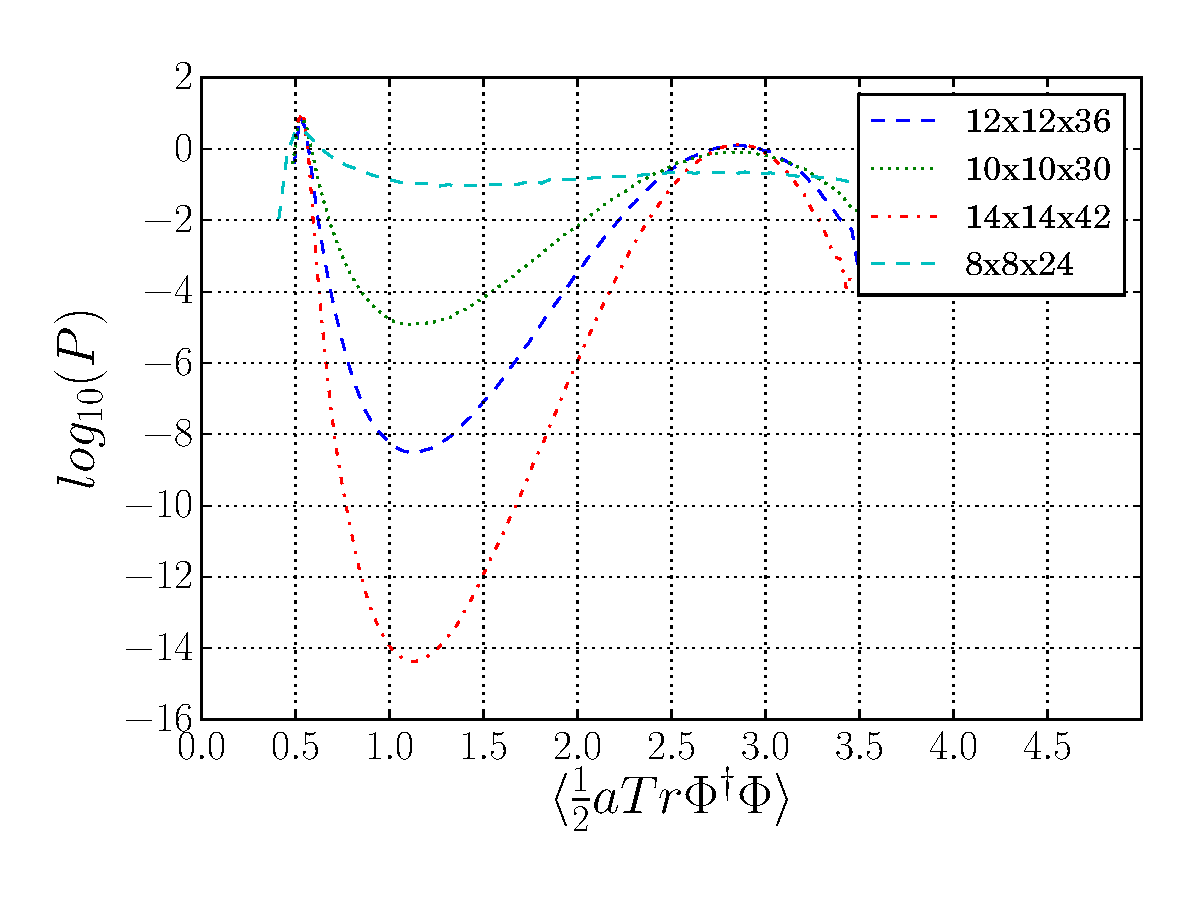
\includegraphics[scale=0.5]{hgrams_beta8_mH35}
	\caption{Histograms for the SM case with inputs as in Eq.~(\ref{eq:SM-inputs}). The smallest volume was done without multicanonical. The histograms agree well with those in Fig.~6 of Ref.~\cite{Kajantie:1995kf}, although our normalization is still off here. Their $\beta_H = 0.3450806$ here, so converting their x-axis to ours using Eq~(\ref{eq:kari_fields}) we see that the peaks are located exactly as in their figure. }
\label{fig:SM_hgrams}
\end{figure}


For the right-hand side histogram in Fig.~6 of Ref.~\cite{Kajantie:1995kf}, the inputs corresponding to $\beta_G=8, m^*_H = 70$ GeV, $T^* = 153.620$ GeV are
\begin{align}
\label{eq:SM-inputs2}
\lambda = 0.0448519 \quad m^2_\text{\phi} = -0.287506.
\end{align}
\lauri{For David's code again $g = 0.707107$.}


\subsection{$\gr{SU(2)} + $adjoint scalar in 3d}

We can compare to histograms in Fig~4 of Ref.~\cite{Kajantie:1997tt}. In this case $\Sigma^a$ is identified as the temporal scalar $A_0^a$ originating from thermal screening of the gauge field $A^a_\mu$. They define 
\begin{align}
	y = \frac{m^2_D(g^2)}{g^4}, \quad x = \frac{\lambda_A}{g^2} = \frac{b_4}{g^2},
\end{align}
in terms of which they give their results (these are in \MSbar!). In Fig.~4 they give $x, \beta_G$ and volume for the histograms, while $y_c$ needs to be calculated from their Eq~(5.12). 

show histograms but only give the critical $y_c$ for the case $x=0.20$, in Fig.~2. Their volume is also quite large, $28^3$, and we need multicanonical in order to simulate this volume. Nevertheless, reading off the critical $y$ corresponding to this volume and $\beta_G = 16$ from their Fig.~2, we have $y_c \approx 0.154$. This fixes the continuum mass $\mu^2_\Sigma$ in our parameterization. 



Their volume in the $x=0.20$ histogram is $28^3$ and the mixed-phase suppression quite strong, so we need a working multicanonical update for the adjoint to compare this case. With just standard metropolis we may nevertheless use smaller volume, $8^3$, and preliminary simulations are in some agreement with their critical values. 


Applying this, we obtain lattice parameters for David's code corresponding to their $x=0.20$ critical histogram: 
\begin{align}
g_\text{latt} = 0.5, \quad b_\text{4,latt}= 0.05, \quad m^2_\text{\Sigma, latt} = -0.315315.
\end{align}


Histograms in Ref.~\cite{Kajantie:1997tt} are given in terms of $A^a_0 A^a_0 / (2 g^2)$ (I don't know if this is the lattice $A^a_0$ or not!!). The condensate discontinuity in their histograms is related to David's histograms by 
\begin{align}
\Delta \langle a \Sigma^a_0\Sigma_0^a\rangle_\text{David} = \frac{8}{\beta_G} \Big(\frac{\Delta\langle A^a_0A_0^a\rangle}{2g^2}\Big)_\text{Kari}.
\end{align}




\subsection{Comparing to Kari's simulations in Higgs + $A_0$ theory}

We can compare the full fundamental + adjoint case to the histograms in Fig.~23 of Ref.~\cite{Kajantie:1995kf}, with $\Sigma$ again being the $A_0$ field. Our DR suggests that the parameters need to be fixed (in terms of 4d parameters) as 
\begin{align}
\mu^2_\Sigma =& m^2_D = g_4^2 T^2 \left( \frac{5}{6} + \frac{N_f}{3} \right) , \quad b_4 = T \frac{g_4^4}{16\pi^2} \left( \frac{17+N_f}{3} \right), \nonumber \\
\quad a_2 =& 2 h_3 = \frac12 g^2_4 T \Big[ 1 + \frac{1}{16\pi^2} \Big( \frac{17}{2} - 4 (4 \ln 2 -1 ) \Big)g_4^2 - 6 y_t^2 + 12\lambda_4 \Big]
\end{align}
These follow simply from 1-loop DR in the SM. However, this is not quite what they use in Ref.~\cite{Kajantie:1995kf}, instead they have made some approximations.

Converting their action to our notation, we see that their $a_2$-term reads 
\begin{align}
\sum_{\textbf{x}} \frac14 a g^2 (a A^a_0 A^a_0) (a \phi^\dagger\phi),
\end{align}
i.e. they fix $h_3 = \frac12 a_2 = \frac14 g_3^2$, which is just the leading-order result from DR.

Performing a similar conversion for the $b_4$ term, we find that their quartic coupling is
\begin{align*}
\beta^A_4 = 4 \frac{b_4}{g^4_3 a},
\end{align*}
and judging from Ref.~\cite{Farakos:1994kx} it seems that they fix 
\begin{align}
b_4 \equiv \lambda_A = \frac{17 g_4^4 T}{48\pi^2},
\end{align}
i.e. they ignore the fermionic contribution from DR. Similarly their mass in the continuum seems to be simply 
\begin{align}
m^2_D = \frac56 g^2_4 T^2. 
\end{align}
\textbf{Note that all parameters in the $A_0$ sector are quite small, and the doublet will dominate the simulations.} Nevertheless, to my knowledge there are no other simulations in the literature performed with both Higgs and an adjoint scalar.

Now for some complications: in Ref.~\cite{Kajantie:1995kf} they do not actually list the explicit input parameters for the $A_0$ simulations. They they values for $m^*_H$ and $T^*$, but only give the relations to $x,y$ in terms of these \textbf{in the case of a fundamental Higgs only}, i.e. the relations already include the integration over $A_0$. So we need to figure out what they used for $x,y$ in this case. 
\begin{comment}
Starting from their parameters in 4d, 
\begin{align}
g_4 &= \frac23 \\ 
h &= \frac{m_H^*}{80.6 \text{ GeV}} \\
\lambda_4 &= \frac18 g_4^2 h^2 ,
\end{align}
we find, using the simplified DR of Ref.~\cite{Farakos:1994kx},
\begin{align}
g^2_3 &= \Big(\frac23\Big)^2 T^* \\
\lambda_3 &= 0.055556 h^2 T^* \\
\mu^2_{\phi,3} &= -\frac12 {m_H^*}^2 + (0.0951588 + 0.0300915 h^2 - 0.000366074 h^4) {T^*}^2.
\end{align}

For their $T^*=170.0$, $m^*_H = 79.976$ GeV, $\beta_G=12$ in Table~9 of \cite{Kajantie:1995kf}, this reciple leads to the following inputs:
\begin{align}
\label{eq:inputs-A0}
g_\text{David} =& 0.57735 \quad \lambda_\text{David} = 0.0410243 \quad a_\text{2, David} = 0.1666667 \nonumber \\ 
b_\text{4,David} =& 0.00531623 \quad m^2_\text{\phi, David} = -0.262436 \quad m^2_\text{\Sigma, David} = -0.228026.
\end{align}


\begin{figure}[h]
	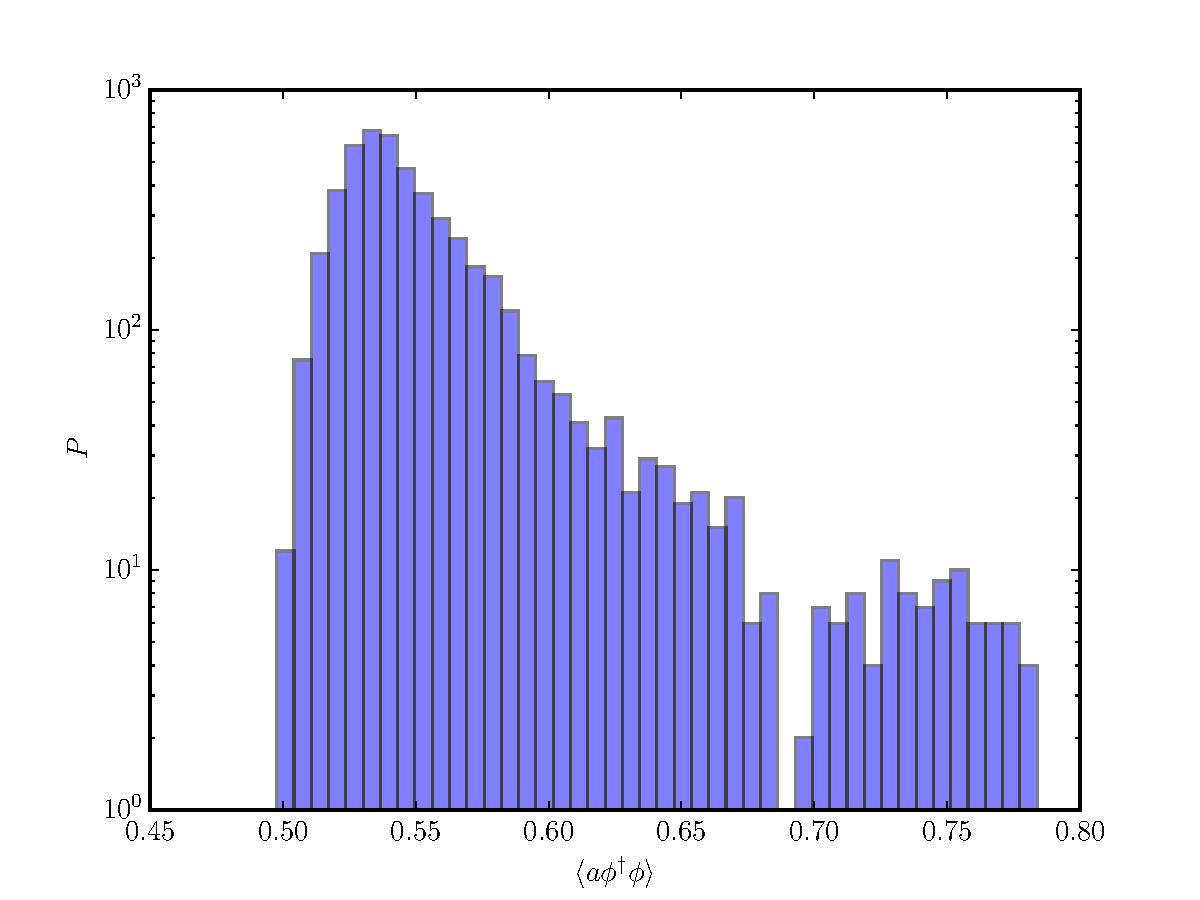
\includegraphics[scale=0.5]{histogram_A0}
	\caption{Histogram for the SM + $A_0$ case with inputs as in Eq.~(\ref{eq:inputs-A0}), at volume $20^3$. The shape is a bit different from Kari's histogram in Fig.~23, but this may be explained by the ambiguity in inputs. Nevertheless we are very close to a transition point here. Again, the separation of peaks agrees quite well with what Kari has. To do: verify this case with multicanonical. }
\end{figure}


\subsection{Updated inputs}

\end{comment}

I asked Kari to search through his old files and he found the following inputs for the fundamental + adjoint case:
\begin{align}
\beta_G = 12, \quad \beta_R = 0.00124, \quad \beta^A_2 = 1.136, \quad \beta^A_4 = 0.1914, 
\end{align}
with only $\beta_H$ varying. According to Ref.~\cite{Kajantie:1995kf} the $A_0$ histograms there are evaluated at $\beta_H = 0.34771$. In terms of these, a straightforward conversion to our lattice parameters gives: 
\begin{align}
m^2_\text{\phi} &= 2\left( \frac{1}{\beta_H} - 3 - \frac{2\beta_R}{\beta_H}\right) = -0.262345\\
\lambda &= \frac{4\beta_R}{\beta_H^2} = 0.0410249 \\
m^2_\text{\Sigma} &= -\frac{2\beta_2^A}{\beta_G} = -0.189333 \\
b_\text{4} &= \frac{4\beta_4^A}{\beta_G^2} = 0.00531667 \\
a_\text{2} &= \frac{2}{\beta_G} = \frac16 = 0.16666667.
\end{align}


\appendix 

\section{Lattice-continuum relations}
\label{sec:lat-cont}

Due to renormalization scheme dependence, the relation between continuum and lattice parameter is nontrivial. In a superrenormalizable 3d theory, \MSbar masses run at two loops while dimensionless couplings are RG invariant. Furthermore, the condensates such as $\langle \phi^\dagger\phi \rangle$ are scheme dependent and need to be matched, although their renormalization is additive and does not affect differences (which are sufficient for extracting the physics). In practice the condensates can be matched by calculating the unphysical zero-point divergence of the effective potential. The schemes can be matched exactly at two loop level, so that the lattice-continuum relations do not obtain further corrections at higher orders. This has been done in Refs.~\cite{Laine:1995np, Laine:1997dy} for the SM and some extensions. Here we collect the results relevant for our cases.

Denoting $m_i = \text{lattice mass}, \mu_i = \text{\MSbar mass}$, the two are related as 
\begin{align}
m^2_i = \mu^2_i(\Lambda) + \delta m^2_i(\hbar) + \delta m^2_i(\hbar^2),
\end{align}
where $\hbar$ is the loop counting parameter. Constants often appearing in the counterterms read \cite{Laine:1997dy}: 
\begin{align}
\Sigma \approx& 3.17591153625, \quad \zeta \approx 0.08849, \quad \delta \approx 1.942130, \quad \rho \approx -0.313964, \nonumber \\ 
\quad \kappa_1 \approx& 0.958382, \quad \kappa_2 = \frac{\Sigma^2}{4} - \frac{\delta}{2} - \frac14, \quad \kappa_3 \approx 0.751498, \quad \kappa_4 \approx 1.204295.
\end{align}
We will denote the \MSbar scale in 3d by $\Lambda$ and the 3d parameters are assumed to be in natural 3d units (e.g. $g^2$ has dimension GeV).

\subsection{$\gr{SU(2)}$ + fundamental Higgs}

The relation between lattice and continuum Higgs condensates is 
\begin{align}
\langle \frac12\Tr\he\Phi\Phi\rangle_\text{cont} = \langle\phi^\dagger\phi\rangle_\text{cont} = \langle \frac12\Tr\he\Phi\Phi\rangle_\text{latt} + \frac{d(\delta V)}{dm^2_\phi}, 
\end{align}
where 
\begin{align}
\label{eq:vacuumCT_higgs}
\delta V =& - 2 m^2_\phi \frac{\Sigma}{4\pi a} - \frac{3}{16\pi^2} g^2 m^2_\phi \Big( \ln \frac{6}{a \Lambda} +\zeta + \frac{\Sigma^2}{4} - \delta \Big).
\end{align}

The full mass counterterm is
\begin{align}
(\delta m^2_\phi)_\text{fund} =& -(\frac32 g^2 + 6\lambda) \frac{\Sigma}{4\pi a} \nonumber \\
&- \frac{1}{16\pi^2}\Big[ \Big( \frac{51}{16}g^4 + 9\lambda g^2 - 12\lambda^2 \Big)\Big( \ln \frac{6}{a\Lambda}+\zeta \Big)
 + 9\lambda g^2 \Big( \frac14 \Sigma^2 - \delta \Big) \nonumber \\ 
& + \frac34 g^4 \Big( \frac{15}{16}\Sigma^2 + \frac{\pi}{3} \Sigma + \frac54 - \frac72 \delta - 4\rho +4\kappa_1 - \kappa_2 - \kappa_3 - 3\kappa_4  \Big) \Big].
\end{align}


\subsection{$\gr{SU(2)}$ + adjoint scalar}

The triplet condensate, we have:
\begin{align}
\frac12 \langle \Sigma^a\Sigma^a\rangle_\text{cont} = \langle\Tr \Sigma^2\rangle_\text{cont} = a^{-1} \langle \Tr \Sigma^2 \rangle_\text{latt} + \frac{d(\delta V)}{dm^2_\Sigma},
\end{align}
where the counterterm is the sum of
\begin{align}
\label{eq:vacuumCT_adj}
\delta V(\hbar) =& -\frac32 m^2_\Sigma \frac{\Sigma}{4\pi a} \nonumber \\
\delta V(\hbar^2) =& -\frac{1}{16\pi^2} 6g^2 m^2_\Sigma \Big( \ln \frac{6}{a \Lambda} +\zeta + \frac{\Sigma^2}{4} - \delta\Big).
\end{align}

The mass counterterm is the sum of
\begin{align}
(\delta m^2_\Sigma(\hbar))_\text{adj} =& -(4g^2 + 5 b_4) \frac{\Sigma}{4\pi a}, \\
(\delta m^2_\Sigma(\hbar^2))_\text{adj} =& -\frac{1}{16\pi^2} \Big[ \Big( 20 b_4 g^2 - 10 b^2_4 \Big)\Big( \ln\frac{6}{a \Lambda} + \zeta \Big) +20 b_4 g^2 \Big( \frac14 \Sigma^2 - \delta \Big) \nonumber \\
 &+ 2 g^4 \Big( \frac54 \Sigma^2 + \frac{\pi}{3}\Sigma - 6\delta -6\rho + 4\kappa_1 -\kappa_2 - \kappa_3 - 3\kappa_4 \Big) \Big].
\end{align}
Note that Ref.~\cite{Laine:1995np} writes the adjoint as $A_0 = A^a_0 \sigma_a$, so their covariant derivative term has different factors of $2$ than we do. Overall the actions are still equivalent. Their parameters are simply $m_D = m_\Sigma, \lambda_A = b_4$.


\subsection{$\gr{SU(2)}$ + fundamental Higgs + adjoint scalar}

The vacuum divergence is not modified by the $a_2$ term, so the counterterm relating the condensates is simply the sum of Eqs.~(\ref{eq:vacuumCT_higgs}) and (\ref{eq:vacuumCT_adj}):
\begin{align}
\delta V =& - ( 2 m^2_\phi + \frac32 m^2_\Sigma ) \frac{\Sigma}{4\pi a} - \frac{3}{16\pi^2} g^2 ( m^2_\phi + 2 m^2_\Sigma ) \Big( \ln \frac{6}{a \Lambda} +\zeta + \frac{\Sigma^2}{4} - \delta \Big).
\end{align}

For the masses, we have 
\begin{align}
m^2_\phi =& \mu^2_\phi(\Lambda) + (\delta m^2_\phi)_\text{fund}+ (\delta m^2_\phi)_\text{both} \\
m^2_\Sigma =& \mu^2_\Sigma(\Lambda) + (\delta m^2_\Sigma)_\text{adj} + (\delta m^2_\Sigma)_\text{both} 
\end{align}
where the new contributions read
\begin{align}
(\delta m^2_\phi)_\text{both} =& -\frac32 a_2 \frac{\Sigma}{4\pi a} - \frac{1}{16\pi^2} \Big[ \Big( -\frac34 g^4 + 6 a_2 g^2 - \frac32 a_2^2  \Big)\Big( \ln \frac{6}{a\Lambda}+\zeta \Big) \nonumber \\ 
& + 6 a_2 g^2 \Big( \frac14 \Sigma^2 - \delta \Big) - 3g^4 \rho \Big], \\
%
(\delta m^2_\Sigma)_\text{both} =& -2 a_2 \frac{\Sigma}{4\pi a} - \frac{1}{16\pi^2}\Big[ \Big( -g^4 + 3 a_2 g^2 - 2 a_2^2 \Big)\Big( \ln\frac{6}{a \Lambda} + \zeta \Big) \nonumber \\
&+ 3 a_2 g^2 \Big( \frac14 \Sigma^2 - \delta \Big) - 4 g^4 \rho \Big].
\end{align}
Note that there are also contributions not proportional to $a_2$.


\section{Code technicalities}

\begin{itemize}
	
	\item Dimensions of spacetime and the lattice size are not fixed beforehand; they are to be read in from config. Our lattice is a $L_1 \times L_2 \times \dots \times L_n$ sized periodic hypercube. It is recommended to use even numbers for $L_i$; otherwise checkerboard updating is not well defined. 
	
	\item We use a single index $i$ to label lattice sites and use this index to access field values etc, instead of Cartesian $(x, y, z, \dots)$ coordinates (these are used in initial layouting). In short, sites are ordered so that the site at origin $(0, 0, 0, \dots)$ has $i = 0$ ("upper left corner"), next site in positive direction $1$ has $i = 1$ etc. When we reach last site in direction $1$, we move one step in direction $2$ and repeat, and so on. Neighbor sites are stored in lookup tables before starting the simulation. \textbf{Update 23.8.2019:} Added routines in layout.c to further reorder the sites by parity. This allows for more optimized update sweeps (in quick test runs the improvement was $20\%$!). The full ordering using this option is: 1. even sites 2. odd sites 3. even halos 4. odd halos. To do: check if memory configuration could be optimized as well with parity ordering.
	
	\item Fields are dynamic arrays of doubles (double*, double**, double***) that are accessed as field[site index][direction][component] for gauge links, field[site index][component] for non-gauge fields. Gauge singlets are simply field[site]. Memory for fields is allocated contiguously. 
	
	\item OpenMPI is used for parallelization. The lattice is split into hypercubes of equal sizes with side lengths $L^\text{slice}_i$, and these are then laid out based on their MPI ranks with same indexing logic as for lattice sites. We treat each node as being a hypercube with side lengths $L^\text{slice}_i + 2$, where the two extra sites are halos that need to be updated using MPI communications. Halo site indexes come after real sites, but otherwise follow same ordering logic. Due to periodicity, it can happen that the physical site corresponding to a halo is actually a real site in the same node. These "self halos" are removed by simply changing the neighbor lookup table to point to the real site instead. All this is implemented in layout.c. 
	
	\item Communication between nodes is implemented in comms.c. We use a "comlist" structure to store information of what site indices our node is supposed to send to which nodes, and what halo site indices do we update with data received from them. Send/receive data is copied into temporary buffers each time we update halos. Each update, we first send our data to all neighbors using nonblocking sends, then proceed with blocking receives to update our halos, and finally wait for all of our sends to go through (usually done by the time we get to the wait loop). Variable c.comms\_time keeps track of the time spent on MPI communications (excluding global multicanonical checks).
	
	\item Updating the lattice is done with checkerboard style sweeps (imagine a chessboard). We specify parity of a site to be EVEN if $x + y + z + \dots $ is an even number, ODD otherwise. When sweeping, we first update all sites with EVEN parity, including halos, and then repeat for ODD sites. Gauge links are updated one direction at a time, because the directions are not independent (think of the Wilson plaquette).  
	
	
\end{itemize}


\begin{thebibliography}{*}


%\cite{Berg:1991cf}
\bibitem{Berg:1991cf}
  B.~A.~Berg and T.~Neuhaus,
  %``Multicanonical algorithms for first order phase transitions,''
  Phys.\ Lett.\ B {\bf 267} (1991) 249.
  doi:10.1016/0370-2693(91)91256-U
  %%CITATION = doi:10.1016/0370-2693(91)91256-U;%%
  %132 citations counted in INSPIRE as of 21 Aug 2019

%\cite{Laine:1998qk}
\bibitem{Laine:1998qk}
M.~Laine and K.~Rummukainen,
%``The MSSM electroweak phase transition on the lattice,''
Nucl.\ Phys.\ B {\bf 535} (1998) 423
doi:10.1016/S0550-3213(98)00530-6
[hep-lat/9804019].
%%CITATION = doi:10.1016/S0550-3213(98)00530-6;%%
%172 citations counted in INSPIRE as of 21 Aug 2019


%\cite{Kajantie:1995kf}
\bibitem{Kajantie:1995kf}
  K.~Kajantie, M.~Laine, K.~Rummukainen and M.~E.~Shaposhnikov,
  %``The Electroweak phase transition: A Nonperturbative analysis,''
  Nucl.\ Phys.\ B {\bf 466} (1996) 189
  doi:10.1016/0550-3213(96)00052-1
  [hep-lat/9510020].
  %%CITATION = doi:10.1016/0550-3213(96)00052-1;%%
  %363 citations counted in INSPIRE as of 24 Apr 2019
  
%\cite{Kajantie:1997tt}
\bibitem{Kajantie:1997tt}
  K.~Kajantie, M.~Laine, K.~Rummukainen and M.~E.~Shaposhnikov,
  %``3-D SU(N) + adjoint Higgs theory and finite temperature QCD,''
  Nucl.\ Phys.\ B {\bf 503} (1997) 357
  doi:10.1016/S0550-3213(97)00425-2
  [hep-ph/9704416].
  %%CITATION = doi:10.1016/S0550-3213(97)00425-2;%%
  %194 citations counted in INSPIRE as of 24 Apr 2019


%\cite{Kennedy:1985nu}
\bibitem{Kennedy:1985nu}
  A.~D.~Kennedy and B.~J.~Pendleton,
  %``Improved Heat Bath Method for Monte Carlo Calculations in Lattice Gauge Theories,''
  Phys.\ Lett.\  {\bf 156B} (1985) 393.
  doi:10.1016/0370-2693(85)91632-6
  %%CITATION = doi:10.1016/0370-2693(85)91632-6;%%
  %234 citations counted in INSPIRE as of 22 Aug 2019

  %\cite{Farakos:1994kx}
\bibitem{Farakos:1994kx}
  K.~Farakos, K.~Kajantie, K.~Rummukainen and M.~E.~Shaposhnikov,
  %``3-D physics and the electroweak phase transition: Perturbation theory,''
  Nucl.\ Phys.\ B {\bf 425} (1994) 67
  doi:10.1016/0550-3213(94)90173-2
  [hep-ph/9404201].
  %%CITATION = doi:10.1016/0550-3213(94)90173-2;%%
  %254 citations counted in INSPIRE as of 07 May 2019


%\cite{Laine:1995np}
\bibitem{Laine:1995np}
  M.~Laine,
  %``Exact relation of lattice and continuum parameters in three-dimensional SU(2) + Higgs theories,''
  Nucl.\ Phys.\ B {\bf 451} (1995) 484
  doi:10.1016/0550-3213(95)00356-W
  [hep-lat/9504001].
  %%CITATION = doi:10.1016/0550-3213(95)00356-W;%%
  %69 citations counted in INSPIRE as of 24 Apr 2019

%\cite{Laine:1997dy}
\bibitem{Laine:1997dy}
  M.~Laine and A.~Rajantie,
  %``Lattice continuum relations for 3-D SU(N) + Higgs theories,''
  Nucl.\ Phys.\ B {\bf 513} (1998) 471
  doi:10.1016/S0550-3213(97)00709-8
  [hep-lat/9705003].
  %%CITATION = doi:10.1016/S0550-3213(97)00709-8;%%
  %67 citations counted in INSPIRE as of 12 Aug 2019


\end{thebibliography}

\end{document}
